\documentclass[tikz]{standalone}
\usepackage{tikz}
\usetikzlibrary{arrows,decorations.pathmorphing,backgrounds,positioning,fit,petri}
\begin{document}
% 基本的画node,shape指定形状,draw指定虽然没有文字也能显示形状
% 指定坐标应该理解成一种添加一个move-to行为
% node的绘制是延迟的,等主要路径绘制完成后node才会绘制出来
% So, the code (0,2) node [shape=circle,draw] {} means the following: “In the main path, add a
% move-to to the coordinate (0,2). Then, temporarily suspend the construction of the main path while the
% node is built. This node will be a circle around an empty text. This circle is to be drawn, but not filled or
% otherwise used. Once this whole node is constructed, it is saved until after the main path is finished. Then,
% it is drawn.” The following (0,1) node [shape=circle,draw] {} then has the following effect: “Continue
% the main path with a move-to to (0,1). Then construct a node at this position also. This node is also
shown after the main path is finished.” And so on.
\begin{tikzpicture}
    \path ( 0,2) node [shape=circle,draw] {}
    ( 0,1) node [shape=circle, draw] {} 
    ( 0,0) node [shape=circle, draw] {}
    ( 1,1) node [shape=rectangle, draw] {}
    (-1,1) node [shape=rectangle, draw] {};
\end{tikzpicture}

% 使用node 的 at 方法指定坐标,避免用move-to,也没有
% 用到node 总是放在最后一个坐标点这条规则
\begin{tikzpicture}
    \path node at ( 0,2) [shape=circle,draw] {}
    node at ( 0,1) [shape=circle,draw] {}
    node at ( 0,0) [shape=circle,draw] {}
    node at ( 1,1) [shape=rectangle,draw] {}
    node at (-1,1) [shape=rectangle,draw] {};
\end{tikzpicture}
% 使用独立的\node命令,这是\path node的缩写
\begin{tikzpicture}
    \node at ( 0,2) [circle,draw] {};
    \node at ( 0,1) [circle,draw] {};
    \node at ( 0,0) [circle,draw] {};
    \node at ( 1,1) [rectangle,draw] {};
    \node at (-1,1) [rectangle,draw] {};
\end{tikzpicture}
% 定义样式,然后在各个\node上应用样式
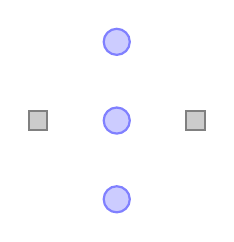
\begin{tikzpicture}
    [place/.style={circle,draw=blue!50,fill=blue!20,thick},
    transition/.style={rectangle,draw=black!50,fill=black!20,thick}]
    \node at ( 0,2) [place] {};
    \node at ( 0,1) [place] {};
    \node at ( 0,0) [place] {};
    \node at ( 1,1) [transition] {};
    \node at (-1,1) [transition] {};
\end{tikzpicture}
% 指定node的大小
% 第一种方案,由于tikz会自动给node里的文字周围添加一些空间,虽然现在文字为空
% 但是这个空间还是存在的,可以用inner sep设置这个空间来控制node的大小
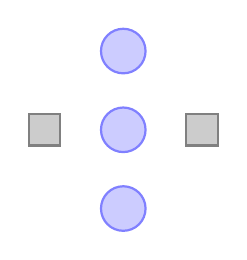
\begin{tikzpicture}
    [inner sep=2mm,
    place/.style={circle,draw=blue!50,fill=blue!20,thick},
    transition/.style={rectangle,draw=black!50,fill=black!20,thick}]
    \node at ( 0,2) [place] {};
    \node at ( 0,1) [place] {};
    \node at ( 0,0) [place] {};
    \node at ( 1,1) [transition] {};
    \node at (-1,1) [transition] {};
\end{tikzpicture}
% 第二种方案,是用minimum size、minimum height、minimum width指定
% 一个node应该有的最小尺寸,如果node里面有文字,他的尺寸还会进一步变大,
% 现在由于没文字,所以就是minimum size。为了确保minimum size设置
% 更精确,这里把inner sep设置为0。
% 两种方式都能设置在style定义里,来让不同的node有不同的尺寸
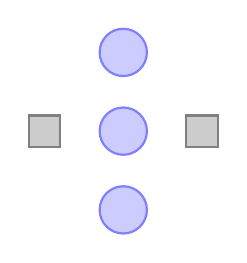
\begin{tikzpicture}
    [place/.style={circle,draw=blue!50,fill=blue!20,thick,
    inner sep=0pt,minimum size=6mm},
    transition/.style={rectangle,draw=black!50,fill=black!20,thick,
    inner sep=0pt,minimum size=4mm}]
    \node at ( 0,2) [place] {};
    \node at ( 0,1) [place] {};
    \node at ( 0,0) [place] {};
    \node at ( 1,1) [transition] {};
    \node at (-1,1) [transition] {};
\end{tikzpicture}
% 给node命名
% 两种方式,一种是用name=的选项,另外一种是直接在node后面加圆括号括起来的名字
% \node 和 {}之间的这些操作的顺序是可以随意变的,不影响结果
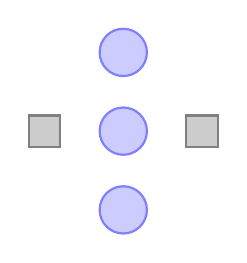
\begin{tikzpicture}
    [place/.style={circle,draw=blue!50,fill=blue!20,thick,
    inner sep=0pt,minimum size=6mm},
    transition/.style={rectangle,draw=black!50,fill=black!20,thick,
    inner sep=0pt,minimum size=4mm}]
    \node (waiting 1) [place]at ( 0,2) {};
    \node (critical 1) [place] at ( 0,1) {};
    \node (semaphore) [place] at ( 0,0) {};
    \node (leave critical) [transition] at ( 1,1) {};
    \node (enter critical) [transition] at (-1,1) {};
\end{tikzpicture}
% 用相对位置来指定node
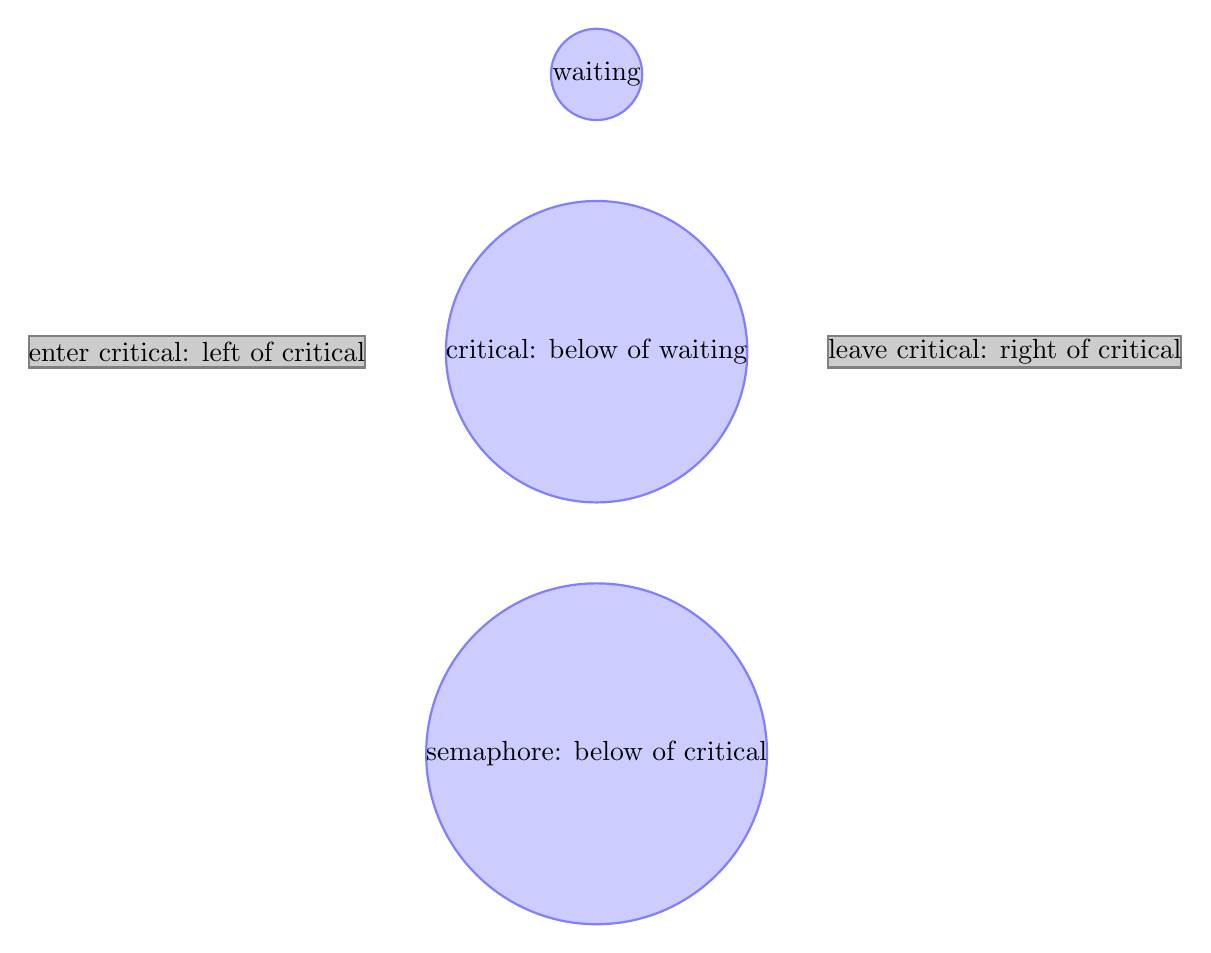
\begin{tikzpicture}
    [place/.style={circle,draw=blue!50,fill=blue!20,thick,
    inner sep=0pt,minimum size=6mm},
    transition/.style={rectangle,draw=black!50,fill=black!20,thick,
    inner sep=0pt,minimum size=4mm}]
    \node[place] (waiting) {waiting};
    \node[place] (critical) [below=of waiting] {critical: below of waiting};
    \node[place] (semaphore) [below=of critical] {semaphore: below of critical};
    \node[transition] (leave critical) [right=of critical] {leave critical: right of critical};
    \node[transition] (enter critical) [left=of critical] {enter critical: left of critical};
\end{tikzpicture}
% 添加标签,两种方式
% 方式一,重新画一个包含标签文字的node,指定其位置
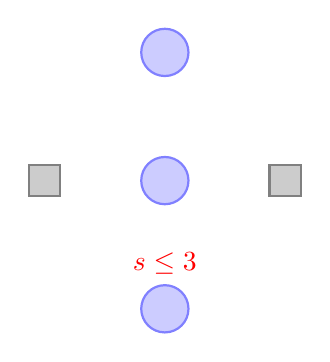
\begin{tikzpicture}
    [place/.style={circle,draw=blue!50,fill=blue!20,thick,
    inner sep=0pt,minimum size=6mm},
    transition/.style={rectangle,draw=black!50,fill=black!20,thick,
    inner sep=0pt,minimum size=4mm}]
    \node[place] (waiting) {};
    \node[place] (critical) [below=of waiting] {};
    \node[place] (semaphore) [below=of critical] {};
    \node[transition] (leave critical) [right=of critical] {};
    \node[transition] (enter critical) [left=of critical] {};
    \node [red,above] at (semaphore.north) {$s\le 3$};
\end{tikzpicture}
% 方式二,直接用node的label选项,相当于自动添加了个node
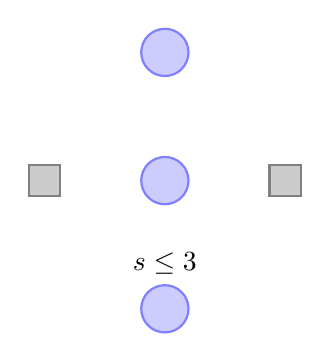
\begin{tikzpicture}
    [place/.style={circle,draw=blue!50,fill=blue!20,thick,
    inner sep=0pt,minimum size=6mm},
    transition/.style={rectangle,draw=black!50,fill=black!20,thick,
    inner sep=0pt,minimum size=4mm}]
    \node[place] (waiting) {};
    \node[place] (critical) [below=of waiting] {};
    \node[place] (semaphore) [below=of critical, label=above:$s\le3$] {};
    \node[transition] (leave critical) [right=of critical] {};
    \node[transition] (enter critical) [left=of critical] {};
\end{tikzpicture}
% 方式二还可以用来添加多个文字标签
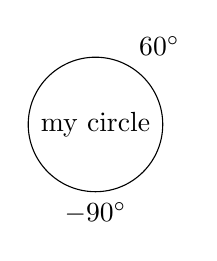
\begin{tikzpicture}
    \node [circle,draw,label=60:$60^\circ$,label=below:$-90^\circ$] {my circle};
\end{tikzpicture}
% 给标签指定颜色,两种方式
% 方式一,指定所有标签的样式
\begin{tikzpicture}[every label/.style={red}]
    \node[place] (waiting) {};
    \node[place] (critical) [below=of waiting] {};
    \node[place] (semaphore) [below=of critical,
    label=above:$s\le3$] {};
    \node[transition] (leave critical) [right=of critical] {};
    \node[transition] (enter critical) [left=of critical] {};
\end{tikzpicture}
% 方式二,为一个标签单独指定颜色
\begin{tikzpicture}
    \node[place] (waiting) {};
    \node[place] (critical) [below=of waiting] {};
    \node[place] (semaphore) [below=of critical,
    label={[red]above:$s\le3$}] {};
    \node[transition] (leave critical) [right=of critical] {};
    \node[transition] (enter critical) [left=of critical] {};
\end{tikzpicture}

% 连接node,通过nodename.anchor的方式可以指定连接线具体接在node
% 的哪个锚点上
\begin{tikzpicture}
    \node[place] (waiting) {};
    \node[place] (critical) [below=of waiting] {};
    \node[place] (semaphore) [below=of critical] {};
    \node[transition] (leave critical) [right=of critical] {};
    \node[transition] (enter critical) [left=of critical] {};
    % critical的西边锚点连上enter critical的东边锚点上
    \draw [->] (critical.west) -- (enter critical.east);
\end{tikzpicture}

% 绘制曲线连接
\begin{tikzpicture}
    \node[place] (waiting) {};
    \node[place] (critical) [below=of waiting] {};
    \node[place] (semaphore) [below=of critical] {};
    \node[transition] (leave critical) [right=of critical] {};
    \node[transition] (enter critical) [left=of critical] {};
    \draw [->] (enter critical.east) -- (critical.west);
    % 指定控制点相对起点和终点的一个偏移的位置
    \draw [->] (waiting.west) .. controls +(left:10mm) and +(up:10mm)
    .. (enter critical.north);
\end{tikzpicture}
% 在连接两个node的时候,tikz能自动的选择锚点,因此上面的指定锚点的
% 过程不是很必要,只有需要特别指定或者tikz不能自动找对锚点时才有必要用
\begin{tikzpicture}
    \node[place] (waiting) {};
    \node[place] (critical) [below=of waiting] {};
    \node[place] (semaphore) [below=of critical] {};
    \node[transition] (leave critical) [right=of critical] {};
    \node[transition] (enter critical) [left=of critical] {};
    \draw [->] (enter critical) -- (critical);
    \draw [->] (waiting) .. controls +(left:8mm) and +(up:8mm)
    .. (enter critical);
\end{tikzpicture}
% 使用to操作进一步简化,in和out选项,能指定连接线出node和
% 入node的时候的角度,不指定时就画直线
\begin{tikzpicture}
    \node[place] (waiting) {};
    \node[place] (critical) [below=of waiting] {};
    \node[place] (semaphore) [below=of critical] {};
    \node[transition] (leave critical) [right=of critical] {};
    \node[transition] (enter critical) [left=of critical] {};
    \draw [->] (enter critical) to (critical);
    \draw [->] (waiting) to [out=180,in=90] (enter critical);
\end{tikzpicture}
% 更简化,使用to的bend left/right选项,这个选项可以理解为从起点到
% 终点的直线路径朝左或是朝右弯曲,角度可以理解为曲线出发时相对直接方向
% 朝左或是朝右偏转了多少,对应的在终点也有一个对称的偏转,
% 角度为0时自然就是直线了。
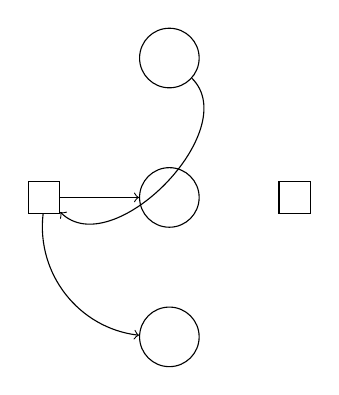
\begin{tikzpicture}
    \node[place] (waiting) {};
    \node[place] (critical) [below=of waiting] {};
    \node[place] (semaphore) [below=of critical] {};
    \node[transition] (leave critical) [right=of critical] {};
    \node[transition] (enter critical) [left=of critical] {};
    \draw [->] (enter critical) to (critical);
    \draw [->] (waiting) to [bend left=90] (enter critical);
    \draw [->] (enter critical) to [bend right=45] (semaphore);
\end{tikzpicture}
% 使用edge操作画连接线,和to操作比较类似,但是有一个重要的区别,
% edge和node一样都不是主要路径的一部分,是在主要路径绘制完成后才
% 进行绘制的,edge也支持bend left/right选项
\begin{tikzpicture}
    \node[place] (waiting) {};
    \node[place] (critical) [below=of waiting] {};
    \node[place] (semaphore) [below=of critical] {};
    \node[transition] (leave critical) [right=of critical] {};
    \node[transition] (enter critical) [left=of critical] {}
    edge [->] (critical)
    edge [<-,bend left=45] (waiting)
    edge [->,bend right=45] (semaphore);
\end{tikzpicture}
% 使用style把edge的bend angle固定,而bend的方向可以具体再指定
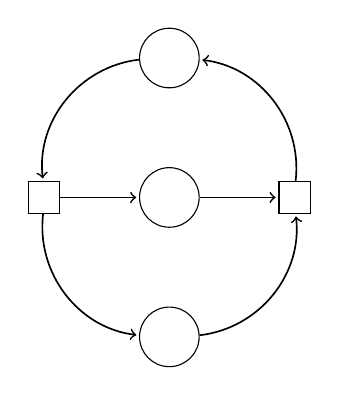
\begin{tikzpicture}
    [bend angle=45,
    pre/.style={<-,shorten <=1pt,semithick},
    post/.style={->,shorten >=1pt,semithick}]
    \node[place] (waiting) {};
    \node[place] (critical) [below=of waiting] {};
    \node[place] (semaphore) [below=of critical] {};
    \node[transition] (leave critical) [right=of critical] {}
    edge [pre] (critical)
    edge [post,bend right] (waiting)
    edge [pre, bend left] (semaphore);
    \node[transition] (enter critical) [left=of critical] {}
    edge [post] (critical)
    edge [pre, bend left] (waiting)
    edge [post,bend right] (semaphore);
\end{tikzpicture}
% 在to操作内添加node作为标签,这样能够把文字标签放在to创建的曲线
% 的中间,auto选项能让node不是压在曲线上面,而是在曲线的一侧,通过
% swap能换到另一侧
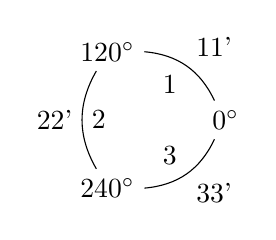
\begin{tikzpicture}[auto,bend right]
    \node (a) at (0:1) {$0^\circ$};
    \node (b) at (120:1) {$120^\circ$};
    \node (c) at (240:1) {$240^\circ$};
    \draw (a) to node {1} node [swap] {11’} (b)
    (b) to node {2} node [swap] {22’} (c)
    (c) to node {3} node [swap] {33’} (a);
\end{tikzpicture}
% 另一个例子,在edge操作内部用node
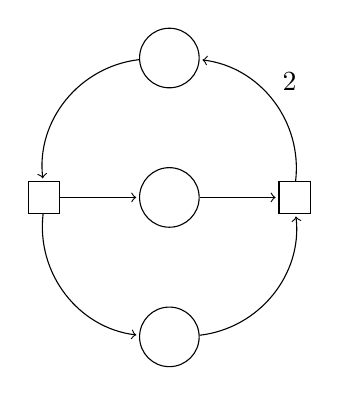
\begin{tikzpicture}[bend angle=45]
    \node[place] (waiting) {};
    \node[place] (critical) [below=of waiting] {};
    \node[place] (semaphore) [below=of critical] {};
    \node[transition] (leave critical) [right=of critical] {}
    edge [pre] (critical)
    edge [post,bend right] node[auto,swap] {2} (waiting)
    edge [pre, bend left] (semaphore);
    \node[transition] (enter critical) [left=of critical] {}
    edge [post] (critical)
    edge [pre, bend left] (waiting)
    edge [post,bend right] (semaphore);
\end{tikzpicture}
% 画蛇形线,decorate表示装饰器,启用蛇形的
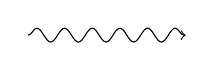
\begin{tikzpicture}
    \draw [->,decorate,decoration=snake] (0,0) -- (2,0);
\end{tikzpicture}
% 上面这种方式会让箭头处看起来比较怪异,可以额外添加一截
% 让结果看起来正常点,post length表示多出来的直线段长度,
% amplitude表示蛇形线的振幅,segment length表示蛇形线的周期
% 所以其实应该是正弦/余弦线

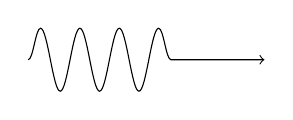
\begin{tikzpicture}
    \draw [->,decorate,
    decoration={snake,amplitude=4mm,segment length=5mm,post length=10mm}]
    (0,0) -- (3,0);
\end{tikzpicture}
% 多行文字标签,实现起来有两种方式
% 方式一,先指定align=center选项,然后使用\\命令在特定位置强制换行
% 如果不指定align=center,换行也不生效
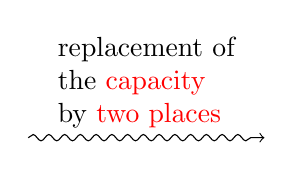
\begin{tikzpicture}
    \draw [->,decorate,
    decoration={snake,amplitude=.4mm,segment length=2mm,post length=1mm}]
    (0,0) -- (3,0)
    node [above,align=left,midway]
    {
    replacement of\\
    the \textcolor{red}{capacity}\\
    by \textcolor{red}{two places}
    };
\end{tikzpicture}
% 方式二,指定文本行的宽度,那么超过宽度就自动换行了
% 而且这种方式下可以不指定对齐方式(align=center等)
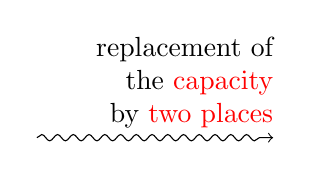
\begin{tikzpicture}
    \draw [->,decorate,
    decoration={snake,amplitude=.4mm,segment length=2mm,post length=1mm}]
    (0,0) -- (3,0)
    node [above,text width=3cm, align=right,midway]
    {
    replacement of the \textcolor{red}{capacity} by
    \textcolor{red}{two places}
    };
\end{tikzpicture}
% 使用layers来实现添加矩形背景的目的
% 由于事先不知道实际网络内容占多大空间,所以先画背景
% 后画网络内容不是一个好的选择。这里可以新开一个作用域,
% 用on background layer来表示这里面的东西都在背景层上
% 然后就可以画一个特定颜色的node,而且tikz还提供了fit操作
% 来免去手动指定尺寸的麻烦,当一个node给了这个操作之后,
% 他会自动的resize和shift来覆盖住参数列表中的其他node
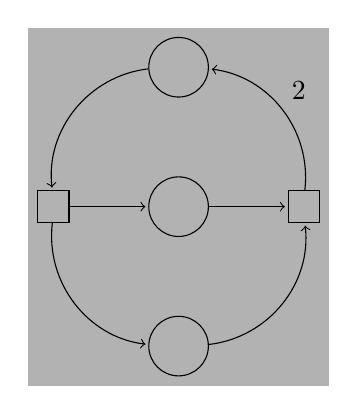
\begin{tikzpicture}[bend angle=45]
    \node[place] (waiting) {};
    \node[place] (critical) [below=of waiting] {};
    \node[place] (semaphore) [below=of critical] {};
    \node[transition] (leave critical) [right=of critical] {}
    edge [pre] (critical)
    edge [post,bend right] node[auto,swap] {2} (waiting)
    edge [pre, bend left] (semaphore);
    \node[transition] (enter critical) [left=of critical] {}
    edge [post] (critical)
    edge [pre, bend left] (waiting)
    edge [post,bend right] (semaphore);
    \begin{scope}[on background layer]
    \node [fill=black!30,fit=(waiting) (critical) (semaphore)
    (leave critical) (enter critical)] {};
    \end{scope}
\end{tikzpicture}
% 关于on background layer再多说两句,就目前的理解来看
% tikz应该有两个层,背景层和前景层,这两个层之间的顺序是
% 前景层始终在背景层之上,而层内部的覆盖关系则是先绘制的
% 在下面,后绘制的在上面。下面的例子中前景层深蓝先画,浅蓝
% 后画,所以浅蓝在上面,背景层中黄色先画,黑色后画,所以
% 黑色在上面,然后前景层的都在背景层的上面,另外背景层
% 必须搭配作用域scope来使用,让作用域内所有的图形都绘制在
% 背景层上,另外还可以给on background layer指定一些选项,
% 这些选项会在作用域内部生效。

\begin{tikzpicture}
    % On main layer:
    \fill[blue] (0,0) circle (1cm);
    \begin{scope}[on background layer={color=yellow}]
    \fill (-1,-1) rectangle (1,1);
    \end{scope}
    \begin{scope}[on background layer]
    \fill[black] (-.8,-.8) rectangle (.8,.8);
    \end{scope}
    % On main layer again:
    \fill[blue!50] (-.5,-1) rectangle (.5,1);
\end{tikzpicture}

% 最后是Petri网教程的最终结果的完整代码
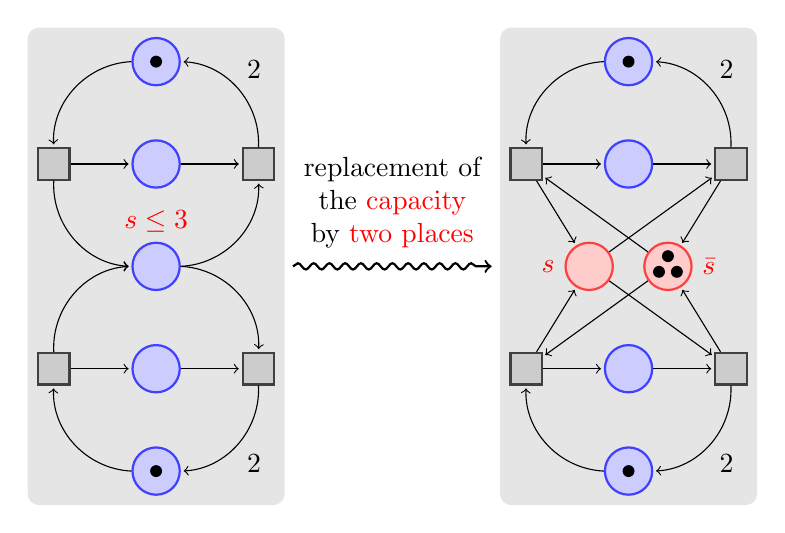
\begin{tikzpicture}
    [node distance=1.3cm,on grid,bend angle=45,auto,
    every place/.style= {minimum size=6mm,thick,draw=blue!75,fill=blue!20},
    every transition/.style={thick,draw=black!75,fill=black!20},
    red place/.style= {place,draw=red!75,fill=red!20},
    every label/.style= {red}]
    % 先画左半部分的网络
    \node [place,tokens=1] (w1) {};
    \node [place] (c1) [below=of w1] {};
    \node [place] (s) [below=of c1,label=above:$s\le 3$] {};
    \node [place] (c2) [below=of s] {};
    \node [place,tokens=1] (w2) [below=of c2] {};
    \node [transition] (e1) [left=of c1] {}
    edge [pre,bend left] (w1)
    edge [post,bend right] (s)
    edge [post] (c1);
    \node [transition] (e2) [left=of c2] {}
    edge [pre,bend right] (w2)
    edge [post,bend left] (s)
    edge [post] (c2);
    \node [transition] (l1) [right=of c1] {}
    edge [pre] (c1)
    edge [pre,bend left] (s)
    edge [post,bend right] node[swap] {2} (w1);
    \node [transition] (l2) [right=of c2] {}
    edge [pre] (c2)
    edge [pre,bend right] (s)
    edge [post,bend left] node {2} (w2);
    % 开启一个作用域,整体往右移6cm,用来画网络的右半部分
    \begin{scope}[xshift=6cm]
        \node [place,tokens=1] (w1’) {};
        \node [place] (c1’) [below=of w1’] {};
        \node [red place] (s1’) [below=of c1’,xshift=-5mm]
        [label=left:$s$] {};
        \node [red place,tokens=3] (s2’) [below=of c1’,xshift=5mm]
        [label=right:$\bar s$] {};
        \node [place] (c2’) [below=of s1’,xshift=5mm] {};
        \node [place,tokens=1] (w2’) [below=of c2’] {};
        \node [transition] (e1’) [left=of c1’] {}
        edge [pre,bend left] (w1’)
        edge [post] (s1’)
        edge [pre] (s2’)
        edge [post] (c1’);
        \node [transition] (e2’) [left=of c2’] {}
        edge [pre,bend right] (w2’)
        edge [post] (s1’)
        edge [pre] (s2’)
        edge [post] (c2’);
        \node [transition] (l1’) [right=of c1’] {}
        edge [pre] (c1’)
        edge [pre] (s1’)
        edge [post] (s2’)
        edge [post,bend right] node[swap] {2} (w1’);
        \node [transition] (l2’) [right=of c2’] {}
        edge [pre] (c2’)
        edge [pre] (s1’)
        edge [post] (s2’)
        edge [post,bend left] node {2} (w2’);
    \end{scope}
    % 新开作用域绘制背景
    \begin{scope}[on background layer]
        \node (r1) [fill=black!10,rounded corners,fit=(w1)(w2)(e1)(e2)(l1)(l2)] {};
        \node (r2) [fill=black!10,rounded corners,fit=(w1’)(w2’)(e1’)(e2’)(l1’)(l2’)] {};
    \end{scope}
    % 绘制左右半图的蛇形连接线
    \draw [shorten >=1mm,-to,thick,decorate,
    decoration={snake,amplitude=.4mm,segment length=2mm,
    pre=moveto,pre length=1mm,post length=2mm}]
    (r1) -- (r2) node [above=1mm,midway,text width=3cm,align=center]
    {replacement of the \textcolor{red}{capacity} by \textcolor{red}{two places}};
\end{tikzpicture}
\end{document}